\documentclass[tikz,border=5mm]{standalone}
\usepackage{tikz}
\usetikzlibrary{shapes.geometric,arrows.meta,positioning,fit,backgrounds,calc}
\usepackage{amsmath}
\usepackage[utf8]{vietnam}

\definecolor{inputBlue}{RGB}{66,133,244}
\definecolor{inputFill}{RGB}{215,232,255}
\definecolor{hiddenGreen}{RGB}{76,175,80}
\definecolor{hiddenFill}{RGB}{225,245,228}
\definecolor{outputOrange}{RGB}{230,162,60}
\definecolor{outputFill}{RGB}{255,240,218}
\definecolor{dropGray}{RGB}{158,158,158}

\tikzset{
    layerblock/.style={rectangle, rounded corners=4pt, very thick,
        minimum width=1.6cm, minimum height=3cm,
        font=\normalsize\bfseries, align=center},
    opblock/.style={rectangle, rounded corners=3pt, thick,
        minimum width=1.4cm, minimum height=0.5cm,
        font=\scriptsize, align=center},
    arr/.style={-{Stealth[length=3mm,width=2.5mm]}, thick, black!60},
}

\begin{document}
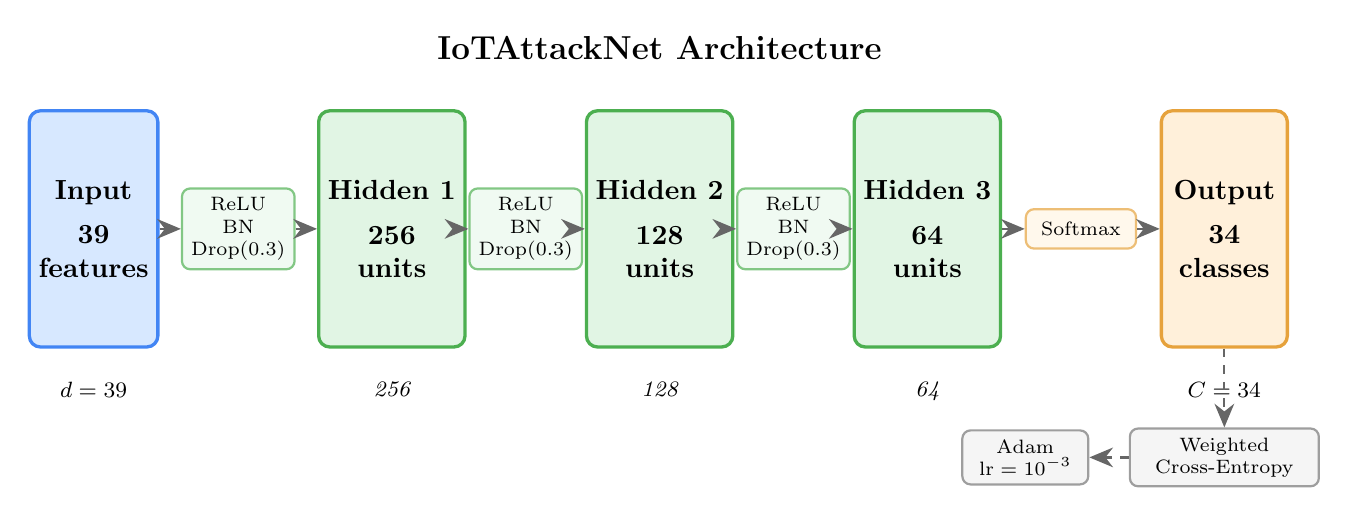
\begin{tikzpicture}[node distance=0.6cm and 1.8cm]

% Input Layer
\node[layerblock, draw=inputBlue, fill=inputFill] (input)
    {\textbf{Input}\\[4pt] 39\\features};

% Hidden Layer 1
\node[layerblock, draw=hiddenGreen, fill=hiddenFill, right=2cm of input] (h1)
    {\textbf{Hidden 1}\\[4pt] 256\\units};

% Hidden Layer 2
\node[layerblock, draw=hiddenGreen, fill=hiddenFill, right=1.5cm of h1] (h2)
    {\textbf{Hidden 2}\\[4pt] 128\\units};

% Hidden Layer 3
\node[layerblock, draw=hiddenGreen, fill=hiddenFill, right=1.5cm of h2] (h3)
    {\textbf{Hidden 3}\\[4pt] 64\\units};

% Output Layer
\node[layerblock, draw=outputOrange, fill=outputFill, right=2cm of h3] (output)
    {\textbf{Output}\\[4pt] 34\\classes};

% Operations between layers
\node[opblock, draw=hiddenGreen!70, fill=hiddenFill!50] at ($(input.east)!0.5!(h1.west)$) (op1)
    {ReLU\\BN\\Drop(0.3)};

\node[opblock, draw=hiddenGreen!70, fill=hiddenFill!50] at ($(h1.east)!0.5!(h2.west)$) (op2)
    {ReLU\\BN\\Drop(0.3)};

\node[opblock, draw=hiddenGreen!70, fill=hiddenFill!50] at ($(h2.east)!0.5!(h3.west)$) (op3)
    {ReLU\\BN\\Drop(0.3)};

\node[opblock, draw=outputOrange!70, fill=outputFill!50] at ($(h3.east)!0.5!(output.west)$) (op4)
    {Softmax};

% Arrows
\draw[arr] (input.east) -- (op1.west);
\draw[arr] (op1.east) -- (h1.west);
\draw[arr] (h1.east) -- (op2.west);
\draw[arr] (op2.east) -- (h2.west);
\draw[arr] (h2.east) -- (op3.west);
\draw[arr] (op3.east) -- (h3.west);
\draw[arr] (h3.east) -- (op4.west);
\draw[arr] (op4.east) -- (output.west);

% Dimension labels
\node[font=\footnotesize\itshape, below=0.3cm of input] {$d = 39$};
\node[font=\footnotesize\itshape, below=0.3cm of h1] {256};
\node[font=\footnotesize\itshape, below=0.3cm of h2] {128};
\node[font=\footnotesize\itshape, below=0.3cm of h3] {64};
\node[font=\footnotesize\itshape, below=0.3cm of output] {$C = 34$};

% Title
\node[font=\large\bfseries, above=0.5cm of h2] {IoTAttackNet Architecture};

% Loss + Optimizer
\node[opblock, draw=dropGray, fill=dropGray!10, below=1cm of output, minimum width=2.4cm] (loss)
    {Weighted\\Cross-Entropy};
\node[opblock, draw=dropGray, fill=dropGray!10, left=0.5cm of loss, minimum width=1.6cm] (optim)
    {Adam\\$\text{lr}=10^{-3}$};
\draw[arr, dashed] (output.south) -- (loss.north);
\draw[arr, dashed] (loss.west) -- (optim.east);

\end{tikzpicture}
\end{document}

